%%%%%%% Unit 2 %%%%%%%%%%
\chapter{Summarizing Data Graphically and Numerically}
\minitoc
\cleardoublepage
\section{Distributions of Quantitative Data}
\inspdfsubsection{Distributions of Quantitative Data: Introduction}{.95}{./pdfs/M4_1}
\inspdfsubsection{Dot Plots}{.95}{./pdfs/M4_2}
\inspdfsubsection{Histograms}{.95}{./pdfs/M4_3}
\subsection{Module 4 Lab}
%\textbf{\large{}Unit 2, Module 4 Lab}{\large \par}
\ \\
\textbf{Name:\hrulefill{}\hspace{0.4\columnwidth}}

\textbf{Learning Goal:} For the distribution of a quantitative variable,
describe the overall pattern (shape, center, and spread) and striking
deviations from the pattern.

\textbf{Specific Learning Objectives:} Compare and contrast the distributions
of a quantitative variable for two groups using histograms. Describe
shape, give a general estimate of center and the overall range, and
calculate relevant percentages.
\begin{enumerate}
\item \textbf{Here are data from adults (247 men and 260 women) who exercise
regularly. The variable is waist girth, measured in centimeters.}\\
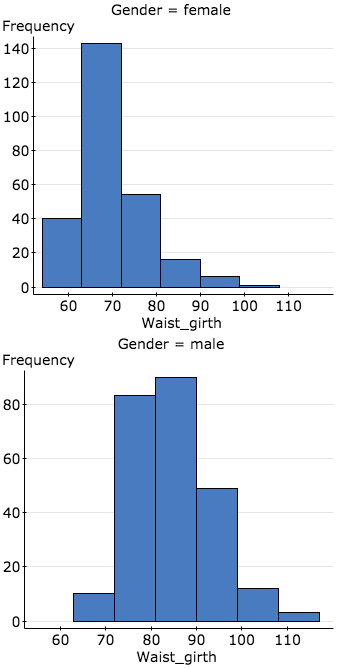
\includegraphics[width=2in]{./img/WaistGirthMF}\\
\textbf{Are the following statements valid (true) or invalid (false)?
Explain how the histograms support your answer.}

\begin{enumerate}
\item In this dataset, typical females have a smaller waist girth than typical
males.\vspace{0.5in}

\item There is less variability in waist girth for females.\vspace{0.5in}

\item Here the distributions of waist girth measurement are skewed to the
right for both males and females, with only a small percentage of
each group having waist girths exceeding 99 cm.\newpage{}
\end{enumerate}
\item \textbf{These histograms show the budget in millions of dollars for
a sample of 74 movies listed in the top 100 USA box offices sales
of all time. The movies are divided into two genres: Action/Adventure
(with 43 movies) and Other (with 31 movies).}\\
\begin{figure}[H]
\noindent \begin{centering}
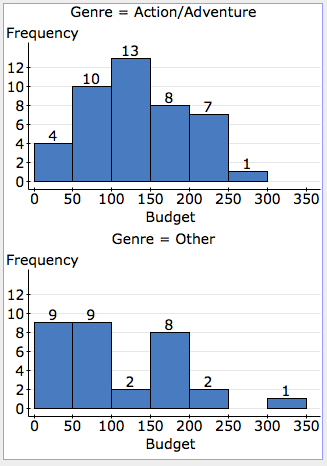
\includegraphics[clip,height=4.5in]{./img/image2}
\par\end{centering}

\end{figure}


\begin{enumerate}
\item Describe the shape of each distribution. What does the shape tell
us about where most of the data fall?\vspace{0.5in}

\item Which genre (Action/Adventure or Other) has the movie with largest
budget?\vspace{0.5in}

\item When we take all of the data into account, which genre tends to have
larger budgets? (To answer this question, give an interval that represents
typical budget amounts for each genre. Use these intervals to support
your answer.)\newpage{}
\item Which genre has more variability in budget amounts? (To answer this
question, estimate the overall range of budget amounts for each genre.
Use your estimates to support your answer.\vspace{0.7in}

\item Pick the statement that you think is more strongly supported by the
data:\\
\begin{figure}[H]
\noindent \begin{centering}
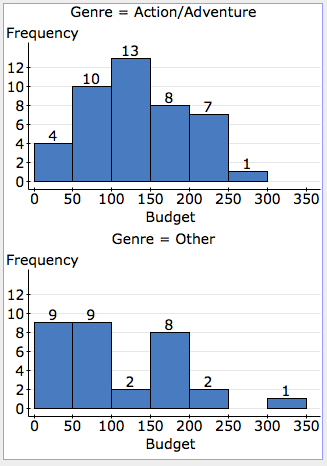
\includegraphics[height=4.5in]{./img/image2}
\par\end{centering}

\end{figure}
\end{enumerate}
\begin{itemize}
\item Action/Adventure movies tend to have larger budgets than other movies.
\item Budget amounts are similar for Action/Adventure movies and Other movies.\\
\\
For the statement you picked, support it with \emph{at least three}
precise observations from the histograms. Explain how your observations
support the statement you chose.\end{itemize}
\end{enumerate}
\clearpage




\cleardoublepage\section{Measures of Center}
\inspdfsubsection{A Feel for Measures of Center}{.95}{./pdfs/centerMedMean}
\inspdfsubsection{The Mean as a Balancing Point}{.95}{./pdfs/meanBalPt}
\inspdfsubsection{Shape and Measures of Center}{.95}{./pdfs/shapeCenterMeas}

\cleardoublepage\section{Measures of Spread about the Median}
\inspdfsubsection{Quantifying Variability Relative to the Median Part 1}{.95}{./pdfs/varMedian1}
\inspdfsubsection{Quantifying Variability Relative to the Median Part 2}{.95}{./pdfs/varMedian2}
\inspdfsubsection{Module 6 Lab}{.95}{./pdfs/U2M6Lab}

\cleardoublepage\section{Quantifying Variability Relative to the Mean}

\inspdfsubsection{Measuring Variability Relative to the Mean: ADM}{.95}{./pdfs/varMean1}
\inspdfsubsection{Using the ADM}{.95}{./pdfs/varMean2}
\inspdfsubsection{The Standard Deviation}{.95}{./pdfs/varMean3}
\inspdfsubsection{The Mean and Standard Deviation: Intervals of Typical Measurements}{.95}{./pdfs/varMean4}
\inspdfsubsection{Module 7 Lab}{.95}{./pdfs/U2M7Lab}
\inspdfsubsection{Unit 2 Summary Lab}{.95}{./pdfs/U2SummaryLab}

\subsection{Unit 2 Project}
%%%%%%%%%%%%%%%% Unit 2 Project %%%%%%%%%%%%%

\textbf{Instructions:} In your group, choose one of the four options described below. Analyze the data using what you have learned in Unit 2. Each group will make a poster and present their analysis in a gallery walk. Based on feedback from the gallery walk, each group will revise their work and present an improved analysis to the class. Your instructor may also require each group member to write an analysis and submit it individually. \\


\textbf{Poster Instructions:} Your poster will include the following: 
\begin{itemize}
\setlength\itemsep{.5pt}
\item A statement of the research question 
\item A description of the source of the data 
\item A description of the variables used in the analysis and an explanation of why your group chose these variables
\item Graphs (with clear labels) and numerical summaries to support your analysis
\item Explanations that reflect the use of Unit 2 concepts
\item An answer to the question based on your analysis of the data
\end{itemize}

\bigskip
\bigskip
\textbf{Option 1: Movies}

\textbf{Research question for Option 1:} Which genres of movies are more successful: Action/Adventure movies or other types of movies? 

Answer this question using the data set \emph{Movies.txt}. Choose at least one quantitative variable that relates to your definition of success. Compare the success of action/adventure movies to other movies using the variable(s) you chose. Follow the instructions for the poster above.


\bigskip
\bigskip
\textbf{Option 2: Body Temperatures}\\

In current medical practice, 98.6�F is considered a normal body temperature, but this is an average.  Normal body temperatures will vary throughout the day and are sensitive to hormone levels. However, an abnormally high or an abnormally low temperature may be a sign of illness. 


\textbf{Research question for Option 2:}
\begin{itemize}
\setlength\itemsep{.5pt}
\item According to this data, what is a normal range for adult body temperature? What temperatures would you label as abnormally high or abnormally low? 
\item Should there be different normal temperature benchmarks for men and women?
\end{itemize} 

To answer these questions analyze the adult body temperature data in \emph{Body Temperature and Heart Rate.txt}. Follow the instructions for the poster above.

\newpage

\textbf{Option 3: Breakfast Cereals}\\

\textbf{Research question for Option 3:} Are cereals targeted at children less healthy than cereals targeted at adults?

Answer this question using the data set \emph{Cereals.txt}. Choose at least one quantitative variable that relates to your definition of healthy or unhealthy. Compare adult and child cereals using the variable(s) you chose. Follow the instructions for the poster above.
\bigskip
\bigskip

\textbf{Option 4: Unisex Belt}\\

Suppose that you are designing a one-size-fits-most unisex belt for adults. The belt should be long enough to fit typical adults without having an excessive amount of extra length. 

\textbf{Research questions for Option 4:}
\begin{itemize} 
\setlength\itemsep{.5pt}
\item What is the length of your belt? Where along the length of the belt are the holes and why?
\item Based on this data, approximately what proportion of adults will be able to wear your belt?
\end{itemize}

Answer these questions using the data set \emph{Body Measurement.txt}. Choose at least one quantitative variable that is relevant to the design of your belt. Follow the instructions for the poster above.

\newpage

\fbox{\begin{minipage}[t]{1\columnwidth}%
\begin{center}
\textbf{\textsc{\large{}Definition Of Variables}}
\par\end{center}%
\end{minipage}}

\textbf{\large{}Option 1: Movies in }\textbf{\emph{\large{}Movies.txt}}{\large \par}

This data set describes 75 movies listed in the top 100 USA box office
sales of all time. Data was taken from IMDb.com in Spring 2014.

\bigskip
\begin{tabbing}
\hspace*{1.8in}\=\kill
\textbf{\emph{Variable}}\> \textbf{Variable Definition}\\
\emph{Year}\> Year\\
\emph{Studio Name}\>Studio Name\\
\emph{Studio Type}\>Studio Type (Big 6, Other)\\
\emph{Genre }\>Genre (Action/Adventure, Other)\\
\emph{Budget (millions \$)}\> Budgeted Cost to Produce (millions \$)\\
\emph{US Box Office (millions \$) }\> US Box Office Revenues (millions\$)\\
\emph{First Week End (millions \$)}\> First Week End Gross Box Office Revenues (millions \$)\\
\emph{Movie\_Length (minutes)}\> Length (minutes)\\
\emph{Trailer\_Length (seconds)}\> Trailer Length (seconds)\\
\emph{Director}\> Name of the Director\\
\emph{Director\_Gender}\> Gender of the Director\\
\emph{Director\_Race}\> Race of the Director\\
\emph{Star}\> Name of the Star\\
\emph{Star\_Gender}\> Gender of the Star\\
\emph{Star\_Race }\> Race of the Star\\
\emph{Costar}\> Name of the Costar\\
\emph{Costar\_Gender }\> Gender of the Costar\\
\emph{Costar\_Race}\> Race of the Costar\\
\emph{IMDb\_Rating}\> How it was rated by IMDb\\
\emph{Metascore}\> How it was rated by Metascore\\
\emph{Metacriticcom\_rating}\> How it was rated by Metacriticcom\\
\emph{Rotten\_Tomatoes}\> How it was rated by Rotten Tomatoes\\
\emph{Number\_of\_Oscars}\> Number of Oscars Won\\
\emph{Oscar\_Nominations}\> Number of Oscar Nominations\\
\emph{Oscar\_Winner}\> Did this movie win an Oscar?\\
\end{tabbing}
\bigskip
\textbf{\large{Option 2: \emph{Body Temperature and Heart Rate.txt}}}

\bigskip
\begin{tabbing}
\hspace*{1in}\=\kill
\textbf{\emph{Variable}}\> \textbf{Variable Definition}\\
\emph{Gender}\> (male, female)\\
\emph{Temperature}\> (degrees F)\\
\emph{Heart Rate}\> (Beats per minute)\\
\end{tabbing}

\newpage
\textbf{\large{Option 3: \emph{Cereals.txt}}}

\bigskip
\begin{tabbing}
\hspace*{1.1in}\=\kill
\textbf{\emph{Variable}}\> \textbf{Variable Definition}\\
\emph{Manufacturer}\>  Manufacturer of cereal\\
\emph{Type}\>  Cereal type (hot or cold)\\
\emph{Shelf}\>  Display shelf at the grocery store\\
\emph{Target}\> Target audience for cereal (Child or Adult)\\
\emph{Calories}\>  Calories per serving\\
\emph{Cups}\>  Number of cups in one serving\\
\emph{Weight}\>  Weight in ounces of one serving\\
\emph{Protein}\>  Grams of protein in one serving\\
\emph{Fat}\>  Grams of fat in one serving\\
\emph{Sodium}\>  Milligrams of sodium in one serving\\
\emph{Fiber}\>  Grams of dietary fiber in one serving\\
\emph{Carbs}\>  Grams of complex carbohydrates in one serving\\
\emph{Sugars}\>  Grams of sugars in one serving\\
\emph{Potassium}\>  Milligrams of potassium in one serving\\
\emph{Vitamins}\>  Vitamins and minerals - 0, 25, or 100\% of daily need in one serving\\
\emph{Rating}\>  Consumer Reports overall rating of nutritional value  \\
\end{tabbing}

\bigskip
\textbf{\large{}Option 4: Body measurements in }\textbf{\emph{\large{}Body
Measurement.txt}}{\large \par}

\bigskip

\begin{tabbing}
\hspace*{1.2in}\=\kill
\textbf{\emph{Variable}}\> \textbf{Variable Definition}\\
\emph{Gender}\>  Gender (male, female)\\
\emph{Age}\>  Age (Years)\\
\emph{Height}\>  Height (Centimeters)\\
\emph{Weight}\>  Weight (Kilograms)\\
\emph{Pelvic\_dia}\>  Pelvic Diameter (Centimeters)\\
\emph{Chest\_depth}\>  Chest Depth (Centimeters)\\ 
\emph{Chest\_dia}\>  Chest Diameter (Centimeters)\\
\emph{Elbow\_dia}\>  Elbow Diameter (Centimeters)\\
\emph{Wrist\_dia}\>  Wrist Diameter (Centimeters)\\
\emph{Knee\_dia}\>  Knee Diameter (Centimeters)\\ 
\emph{Ankle\_dia}\> Ankle Diameter (Centimeters)\\
\emph{Shoulder\_girth}\>  Shoulder Girth (Centimeters)\\
\emph{Chest\_girth }\> Chest Girth (Centimeters)\\
\emph{Waist\_girth}\>  Waist Girth (Centimeters)\\
\emph{Abdominal\_girth}\>  Abdominal Girth (Centimeters)\\
\emph{Hip\_girth}\>  Hip Girth (Centimeters)\\
\emph{Thigh\_girth}\>  Thigh Girth (Centimeters)\\
\emph{Bicep\_girth}\>  Bicep Girth (Centimeters)\\
\emph{Forearm\_girth}\>  Forearm Girth (Centimeters)\\\
\emph{Knee\_girth}\>  Knee Girth (Centimeters)\\
\emph{Calf\_girth}\>  Calf Girth (Centimeters)\\
\emph{Ankle\_girth}\>  Ankle Girth (Centimeters)\\
\emph{Wrist\_girth}\>  Wrist Girth (Centimeters)
\end{tabbing}



